\documentclass[runningheads]{llncs}

\usepackage{amsmath, amssymb}      % For advanced math symbols
\usepackage{bm}                   % For bold math symbols
\usepackage[T1]{fontenc}
\usepackage{graphicx}
\usepackage{url}
\usepackage{subcaption}           % For subfigures
\usepackage{float}
\usepackage{orcidlink}

\begin{document}

\title{Single-Stage Autoencoder for IoT Intrusion and Zero-Day Threat Identification}
\titlerunning{Single-Stage Autoencoder for IoT Intrusion Detection}

\author{Sergio Mart\'in~Reiz\'abal\inst{1}\orcidlink{0009-0001-3284-9100}
\and C\'{e}sar {Rodr\'{i}guez~Villagr\'{a}}\inst{1}\orcidlink{0009-0007-0122-7417}\and Rub\'{e}n Ruiz Gonz\'{a}lez\inst{1}\orcidlink{0000-0001-7006-2395} \and Nu{\~n}o Basurto\inst{1}\orcidlink{0000-0001-7289-4689} }
\authorrunning{S. Mart\'in Reiz\'abal}
\institute{Grupo de Inteligencia Computacional Aplicada (GICAP), Universidad de Burgos, \\
Av. Cantabria s/n, 09006 Burgos, Spain \\
\email{\{smreizabal, ruben.ruiz, nbasurto\}@ubu.es, crv1002@alu.ubu.es}}
\maketitle

\begin{abstract}
This study proposes an enhanced single-stage autoencoder model for simultaneous multiclass attack classification and zero-day attack detection in IoT network traffic. The approach first evaluates the reconstruction error against a predefined threshold to determine whether the network samples represent potential zero-day threats or known categories. Only samples below this threshold are classified using a compressed latent representation, ensuring the efficient and accurate identification of known attack types. This dual-capability design significantly enhances the detection of previously unseen threats (zero-day attacks) while maintaining a robust multiclass classification performance. Experiments were conducted using the UNSW-NB15 dataset to demonstrate the effectiveness of the proposed model, achieving a balance between accurately classifying known attacks and effectively identifying zero-day intrusions. The integration of both reconstruction and classification tasks within a single-stage architecture renders the proposed approach particularly suitable for deployment in resource-constrained IoT environments, where efficiency and rapid threat detection are critical.
% \keywords{Autoencoder \and Intrusion Detection \and IoT Security \and Zero-Day Attacks \and Multi-class Classification \and UNSW-NB15}
\keywords{Intrusion Detection \and Zero-Day Attacks \and Multi-Class Classification \and Hybrid Autoencoder \and Latent Space Optimization}
\end{abstract}

\section{Introduction}
Zero-day attacks exploit previously unknown vulnerabilities, which often remain undetected for extended periods~\cite{bilge_2012}. Recent reports indicate a significant increase in these threats, highlighting the urgent need for real-time Intrusion Detection Systems (IDS), particularly in resource-constrained Internet of Things (IoT) environments. In fact, data from 2023 shows a 50\% increase in zero-day exploits compared to 2022~\footnote{Zero-day exploits jumped 50\% in 2023, fueled by spyware vendors \url{https://therecord.media/zero-day-exploits-jumped-in-2023-spyware}}.

Inspired by Kitsune, a lightweight autoencoder-based IDS~\cite{mirsky_2018}, this study proposes a single-stage autoencoder architecture that integrates both multi-class classification and zero-day threat detection. The model first evaluates the reconstruction error to identify potential zero-day attacks, and subsequently classifies known attack types using latent-space representations.

The proposed approach was validated using the UNSW-NB15 dataset~\cite{moustafa_2015}, thereby demonstrating its ability to accurately classify known attacks while effectively detecting previously unseen threats.

To simulate zero-day attacks, a subset of attack classes (Backdoor, Shellcode, Exploits, and Reconnaissance) was deliberately excluded from the training set and reserved solely for evaluation. This exclusion ensures the detector has no prior exposure to these held-out attack signatures, so any successful identification relies purely on anomaly detection capabilities rather than learned patterns~\cite{10577735}.

Recent reviews categorize machine learning–based zero-day detection methods into five broad paradigms: supervised (e.g., SVM, Random Forest, Decision Trees), unsupervised (e.g., autoencoders, clustering), hybrid combinations of both, federated learning for privacy-preserving distributed detection, and lightweight models optimized for IoT deployments~\cite{10851751}. Our single-stage autoencoder, operating on 5-tuple flow statistics, positions itself as a lightweight hybrid solution capable of both anomaly-based zero-day detection and multiclass attack classification in real time.

\section{Methodology}\label{sec:Methodology}

\subsection{Single-Stage Autoencoder-Based Intrusion Detection}
The proposed approach introduced a single-stage autoencoder architecture that combined anomaly detection and multiclass classification. Initially, the autoencoder computes the reconstruction error, which, compared to a threshold, determines whether the samples represent potential zero-day threats. Samples below the threshold were classified using latent-space representation.

\subsection{Combined Loss Function}
To jointly optimize the reconstruction and classification, the following combined loss function is employed:
\begin{equation}
    \mathcal{L} = \text{MSE}\bigl(X, \hat{X}\bigr) + \alpha \cdot \text{CE}\bigl(y, \hat{y}\bigr)
\end{equation}

where \(\text{MSE}\) is the mean squared error between the input \(X\) and its reconstruction \(\hat{X}\), \(\text{CE}\) is the cross-entropy loss between the ground-truth labels \(y\) and the predicted labels \(\hat{y}\), and \(\alpha\) is a hyperparameter that balances the two components.

\subsection{Zero-Day Attack Detection}
During inference, samples exceeding a predefined reconstruction error threshold based on the training set distribution were flagged as zero-day attacks. The remaining samples were subjected to multiclass classification.

\section{Experimental Setup}
\subsection{Dataset and Data Splitting}
The dataset mentioned above contains diverse network traffic samples labeled with various attack categories. The present study focuses on a subset of attacks by defining
\begin{itemize}
    \item \textbf{Known Classes:} \texttt{Fuzzers}, \texttt{DoS}, \texttt{Generic}, and \texttt{Normal}.
    \item \textbf{Unknown Classes (simulated zero-day):} \texttt{Backdoor}, \texttt{Shellcode}, \texttt{Exploits}, and \texttt{Reconnaissance}.
\end{itemize}
For training, only samples from the known classes were used to train the combined autoencoder classifier (see Section~\ref{sec:Methodology}). The test set includes both known and unknown classes, allowing us to evaluate the multi-class classification performance and assess zero-day detection via reconstruction error.

\section{Model Architecture}

The proposed single-stage architecture integrates zero-day detection and multiclass classification in a single pass. First, the autoencoder computes the reconstruction error of each input against a predefined threshold; samples exceeding the threshold are flagged as potential zero-day attacks and omitted from further classification. If the reconstruction error is below the threshold, the corresponding latent representation is immediately passed to the classification head to predict one of the known attack classes or normal traffic.
\begin{figure}[!htb]
    \centering
    
\includegraphics[width=\textwidth]{Springer Lecture Notes in Computer Science (1)/imgs/Single-Stage-AE.png}
    \caption{Single-stage autoencoder–classifier architecture.}
    \label{fig:model_architecture}
\end{figure}

Figure~\ref{fig:model_architecture} illustrates this end-to-end workflow, where the encoder compresses the input 5-tuple flow statistics into a lower-dimensional latent space, which is used by both the decoder (for reconstruction) and the classification head (for multiclass prediction), conditional on the error check.



\section{Results}

Various values of hyperparameter $\alpha$ were evaluated to balance the model’s classification and zero-day detection capabilities. Table~\ref{tab:known_vs_zero_day} summarizes the balanced accuracy and macro F1 score for known attacks, along with the balanced accuracy and AUC-ROC scores for zero-day detection. The Overall Score metric was defined as the average balanced accuracy across both of the tasks.

\begin{table}[ht!]
\centering
%\tiny
\caption{Comparison of known vs.\ zero-day performance for different values of $\alpha$.}
\label{tab:known_vs_zero_day}
\begin{tabular}{c|cc|cc|c}
\hline
 & \multicolumn{2}{c|}{\textbf{Known Attacks (Validation)}} & \multicolumn{2}{c|}{\textbf{Zero-Day (Test)}} & \textbf{Overall Score} \\
\textbf{$\alpha$} & \textbf{Bal.\ Acc.} & \textbf{Macro F1} & \textbf{Bal.\ Acc.} & \textbf{AUC-ROC} & \textbf{Composite} \\
\hline
0   & 0.1783 & 0.0213 & 0.6050 & 0.6919 & 0.3866 \\
1   & 0.7997 & 0.7171 & 0.6128 & 0.7212 & 0.7542 \\
2   & 0.7982 & 0.7170 & 0.6241 & 0.7585 & 0.7576 \\
3   & 0.7870 & 0.7173 & 0.5661 & 0.7261 & 0.7229 \\
5   & 0.7811 & 0.7217 & 0.5670 & 0.7149 & 0.7212 \\
10  & 0.8016 & 0.7180 & 0.5620 & 0.7502 & 0.7286 \\
\hline
\end{tabular}
\end{table}

As shown in Table~\ref{tab:known_vs_zero_day}, the best overall value of $\alpha$ is 2 (composite score of 0.7576), indicating a good trade-off between classifying known attacks and detecting zero-day samples.

\subsection{Latent Space Analysis}
Figure~\ref{fig:pca_latent} compares the PCA projections of the latent space for different $\alpha$ values. 
In \subref{fig:latent_0} ($\alpha=0$), the model behaves as a pure autoencoder, minimizing only reconstruction error, which results in overlapping classes. 
In \subref{fig:latent_2} ($\alpha=2$), the classification loss enforces better class separation, making \texttt{Generic} (pink) and \texttt{Normal} (light blue) more distinct, whereas \texttt{DoS} and \texttt{Fuzzers} still exhibit some overlap. 
This demonstrates how the combined loss reshapes the latent space and balances zero-day detection with multiclass classification.

\begin{figure}[htbp]
 \centering
 \begin{subfigure}{0.48\textwidth}
     \centering
     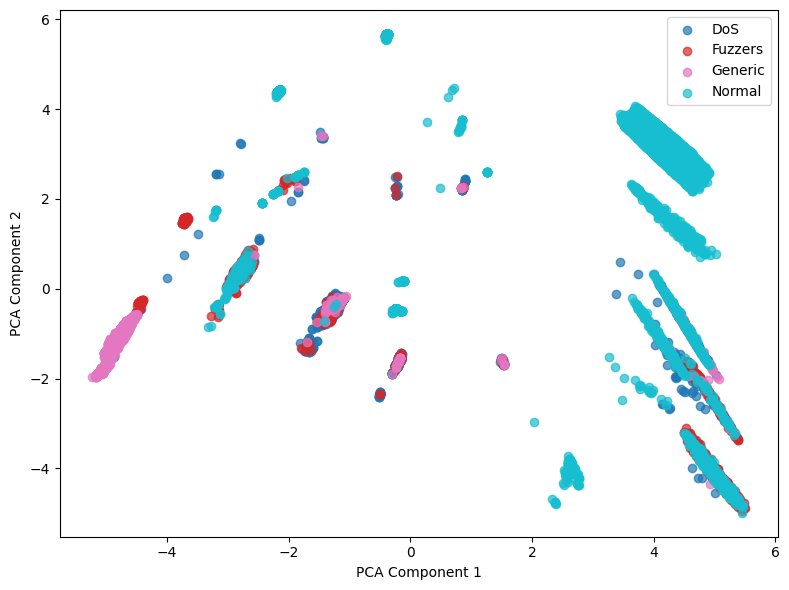
\includegraphics[width=\textwidth]{imgs/latent_0.png}
     \caption{Latent space projection with $\alpha = 0$.}
     \label{fig:latent_0}
 \end{subfigure}
 \hfill
 \begin{subfigure}{0.48\textwidth}
     \centering
     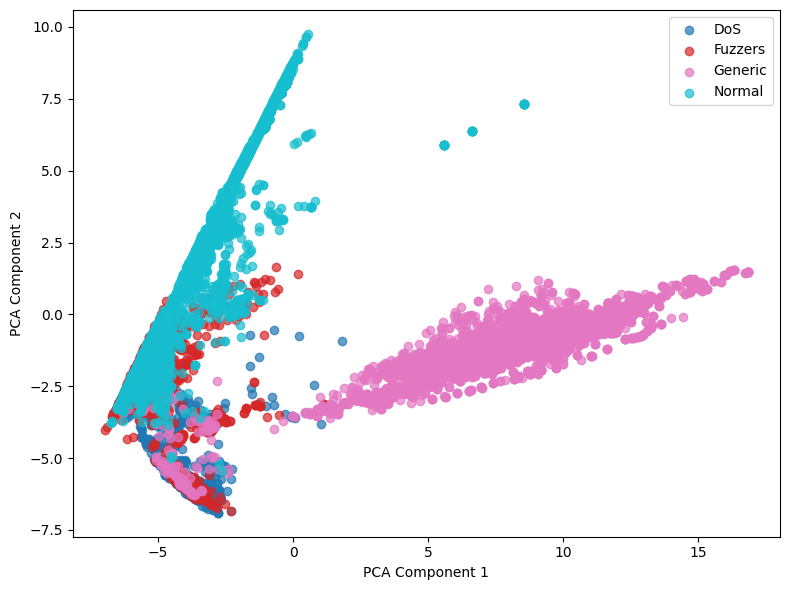
\includegraphics[width=\textwidth]{imgs/latent_2.png}
     \caption{Latent space projection with $\alpha = 2$.}
     \label{fig:latent_2}
 \end{subfigure}
 \caption{PCA projection of the latent space for different values of $\alpha$.}
 \label{fig:pca_latent}
\end{figure}

\subsection{Zero-Day Detection}
To assess the model capability to flag unknown attacks, the reconstruction error was computed on the test set and compared with a threshold derived from the validation distribution. Figure~\ref{fig:error_hist} shows a \emph{violin plot} of the reconstruction error distribution for both known (blue) and zero‑day (red) samples; the dashed line marks the selected threshold ($7.7\!\times\!10^{-3}$).

Quantile analysis highlights the error gap between the two groups.
\begin{itemize}
    \item \textbf{25th percentile (Q1):} Known~$\approx5\!\times\!10^{-4}$; Zero‑Day~$\approx1\!\times\!10^{-3}$ ($\times2$).
    \item \textbf{Median (Q2):} Known~$\approx1\!\times\!10^{-3}$; Zero‑Day~$\approx5\!\times\!10^{-3}$ ($\times5$).
    \item \textbf{75th percentile (Q3):} Known $\approx2\!\times\!10^{-3}$; Zero‑Day $\approx8\!\times\!10^{-3}$ ($\times4$).
\end{itemize}

The threshold cleanly separates most zero‑day samples while preserving the vast majority of known traffic below it.

\begin{figure}[htbp]
    \centering
    %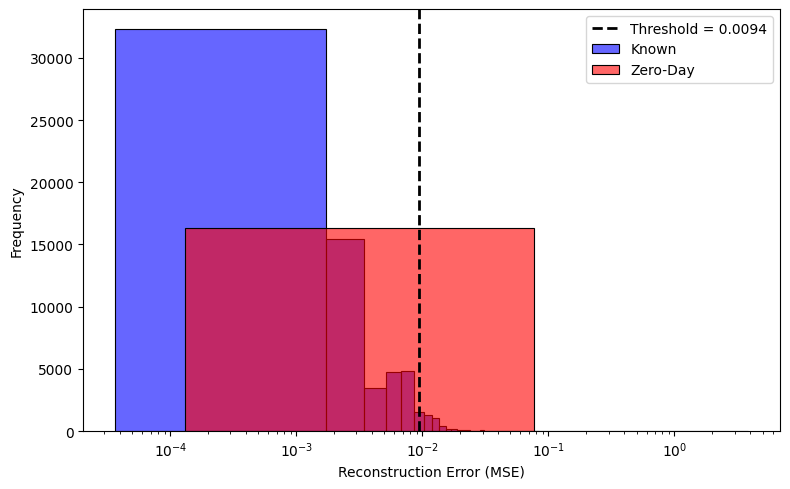
\includegraphics[width=0.55\textwidth]{imgs/error_distribution.png}
    
\includegraphics[width=0.8\textwidth]{Springer Lecture Notes in Computer Science (1)/imgs/ViolinPlot.png}
    \caption{Violin plot of the reconstruction error (MSE) for known (blue) versus zero‑day (red) traffic. The dashed horizontal line denotes the threshold ($7.7\!\times\!10^{-3}$).}
    \label{fig:error_hist}
\end{figure}

\subsection{Discussion}
The experiments demonstrated that combining reconstruction and classification losses allows the model to classify known attacks while detecting zero-day intrusions. As shown in Table~\ref{tab:known_vs_zero_day}, $\alpha=2$ achieves the best balance. Future work could enhance latent space separability through improved architectures or regularization techniques.


\section*{Acknowledgements}
This publication is part of the AI4SECIoT project ("Artificial Intelligence for Securing IoT Devices"), funded by the National Cybersecurity Institute (INCIBE), derived from a collaboration agreement signed between the National Institute of Cybersecurity (INCIBE) and the University of Burgos. This initiative is carried out within the framework of the Recovery, Transformation and Resilience Plan funds, financed by the European Union (Next Generation), the project of the Government of Spain that outlines the roadmap for the modernisation of the Spanish economy, the recovery of economic growth and job creation, for solid, inclusive and resilient economic reconstruction after the COVID‑19 crisis, and to respond to the challenges of the next decade.


\bibliographystyle{splncs04}
\bibliography{references.bib}

\end{document}

% PCA --> CMLHL →